% % Third Chapter : Implementation
%
% Master Thesis: Calibration and Fusion of Stereoscopic and Time-of-Flight 
% Cameras for Zero Gravity Targets Inspection
%
% Achieved at Space System Lab, M.I.T.
% Supervisor: Alvar Saenz-Otero, Daniel Alazard
%
% Institut Sup�rieur de l'A�ronautique et de l'Espace
% Major: Telecommunications et r�seaux - Syst�mes Spatiaux et Lanceurs
% Gabriel Urbain - October 2014
%%

\chapter{Implementation}

\section{Language and Libraries}
The algorithms detailed in the previous chapter have been implemented to be tested with the sensors presented in the first chapter. The choice of \textit{C++} as a programming language came naturally for the following reasons:
\begin{itemize*}
\item This language is used inside the \gls{VERTIGO}, \gls{INSPECT} and \gls{SPHERES} cores.
\item \textit{C++} is the most common language on Linux and Ubuntu 12.04 is the operating system of the \gls{VERTIGO} computer.
\item \textit{C++} benefits from multiple libraries.
\item The cameras constructors provided \textit{C++} API on Linux for their hardware.
\end{itemize*}
To simplify the implementation and avoid useless developments, we also used third-part libraries:
\begin{itemize*}
\item \textit{MESA-Imaging \gls{API}} for the \gls{ToF} camera.
\item \textit{IDS-Imaging uEye \gls{API}} for the stereo cameras.
\item \textit{PLEORA eBUS \gls{SDK}} for the thermographic camera.
\item \textit{OpenCV} for image processing, matrix operations and result display.
\item \textit{Point Cloud Library ()\gls{PCL})} for 3D points cloud manipulation and display.
\item \textit{Boost} for matrix operations and numerical solvers.
\item \textit{Eigen} for matrix operations and numerical solvers.
\end{itemize*}

\section{Software Architecture}
Beside a few tests on Matlab and with \textit{OpenCV} as well as the camera acquisition programming in the \gls{INSPECT} core, this project has focused on a software implementing live and post-processing of images captured by the \gls{ToF} and the stereo devices. The sources and tutorials of this software are available in the repository:
\begin{center}
\texttt{https://github.com/Gabs48/Inspect\_sensor\_fusion}
\end{center}
In its architecture presented in figure \ref{fig:uml}, the classes \textit{Camera}, \textit{ORF} and \textit{Thermocam} directly implement the acquisition using the constructors API. Alternatively, they can be initialized to read files in a directory to perform post-processing instead. \textit{Halo} is a class representing the Halo hardware and implements the \textit{Camera}, the \textit{ORF} and the \textit{Thermocam} devices. Each of those four classes inherits from \textit{Calibration} which allows to compute calibration parameters when they are not available yet in calibration files. \textit{StereoTriangulation} and \textit{OrfTriangulation} implement the projection and triangulation process for the two sensors. Finally, \textit{HaloTriangulation} contains the fusion algorithm itself since it reconstructs 3D points from the sensors data. \textit{Utils} provides a few tools like the \textit{TimeStamp} class to compare acquisition time of sensors between each others.

% figure uml
\begin{figure}[H]
	\begin{center}
		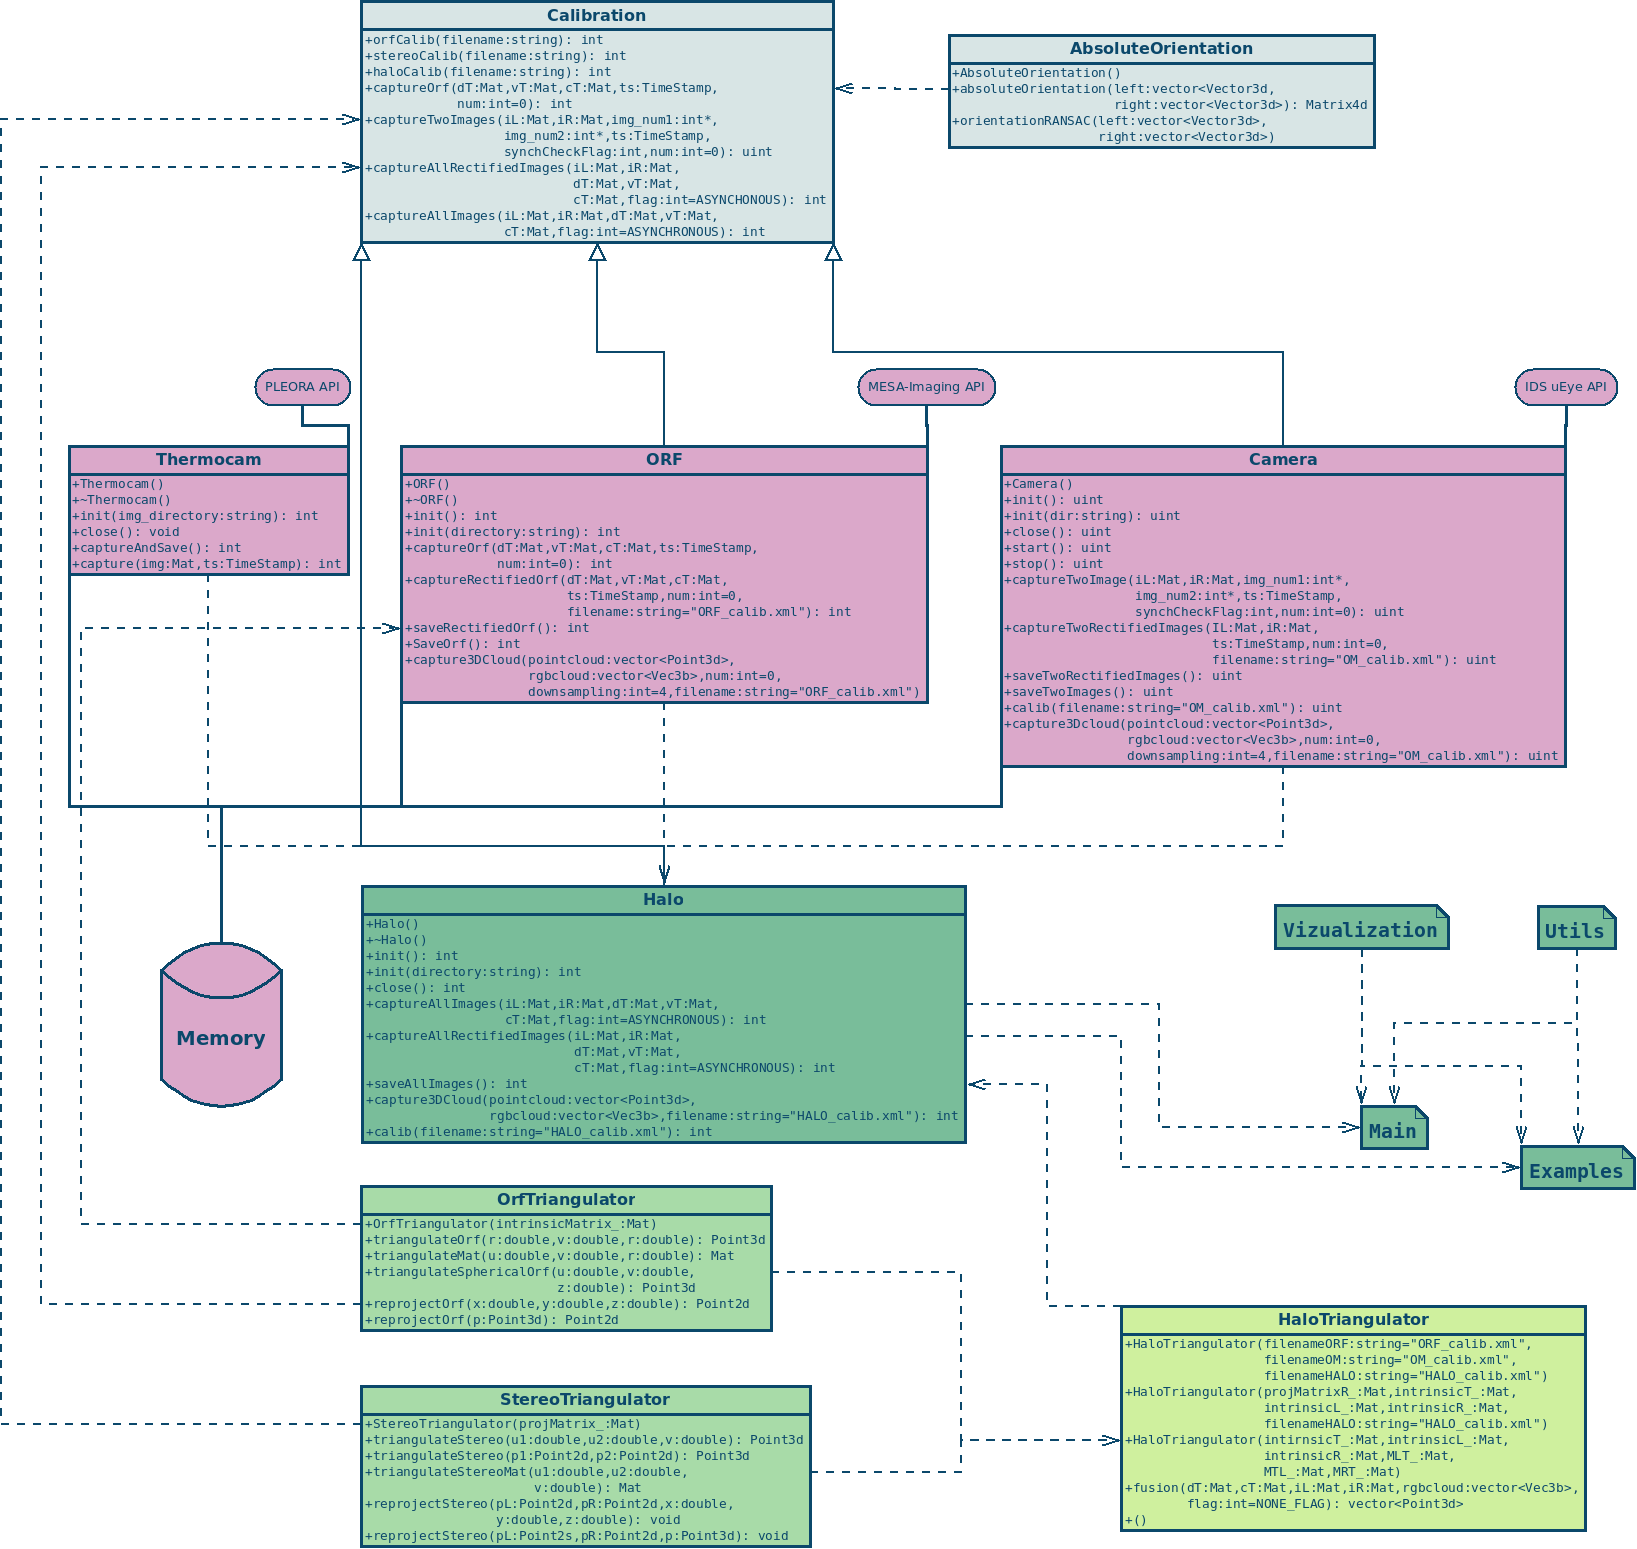
\includegraphics[width=16cm]{img/uml.png}
		\caption{The UML diagram of the Inspect Sensor Fusion software available in the public repository \texttt{https://github.com/Gabs48/Inspect\_sensor\_fusion}. Pink correspond to acquisition classes; Light blue to calibration classes; Very light green to fusion class; Green a bit darker to projection and triangulation classes; Remaining classes are in dark green.}\label{fig:uml}
	\end{center}
\end{figure}

